\section{Controller}

The controller is a Mealy machine used to sequence operations performed on the datapath.
Figure~\ref{fig:ControlBlock} contains all inputs, outputs and internal registers.
There are $7$ labelled inputs including two $4$ bit buses and one $8$ bit bus.
There are $26$ labelled outputs including five $4$ bit buses and one $3$ bit bus.
Typedefs, defined in a global file, are used for some single bit outputs and all bus outputs to keep decoding consistent in control and the datapath. 


\begin{figure}[t]
   \centering
    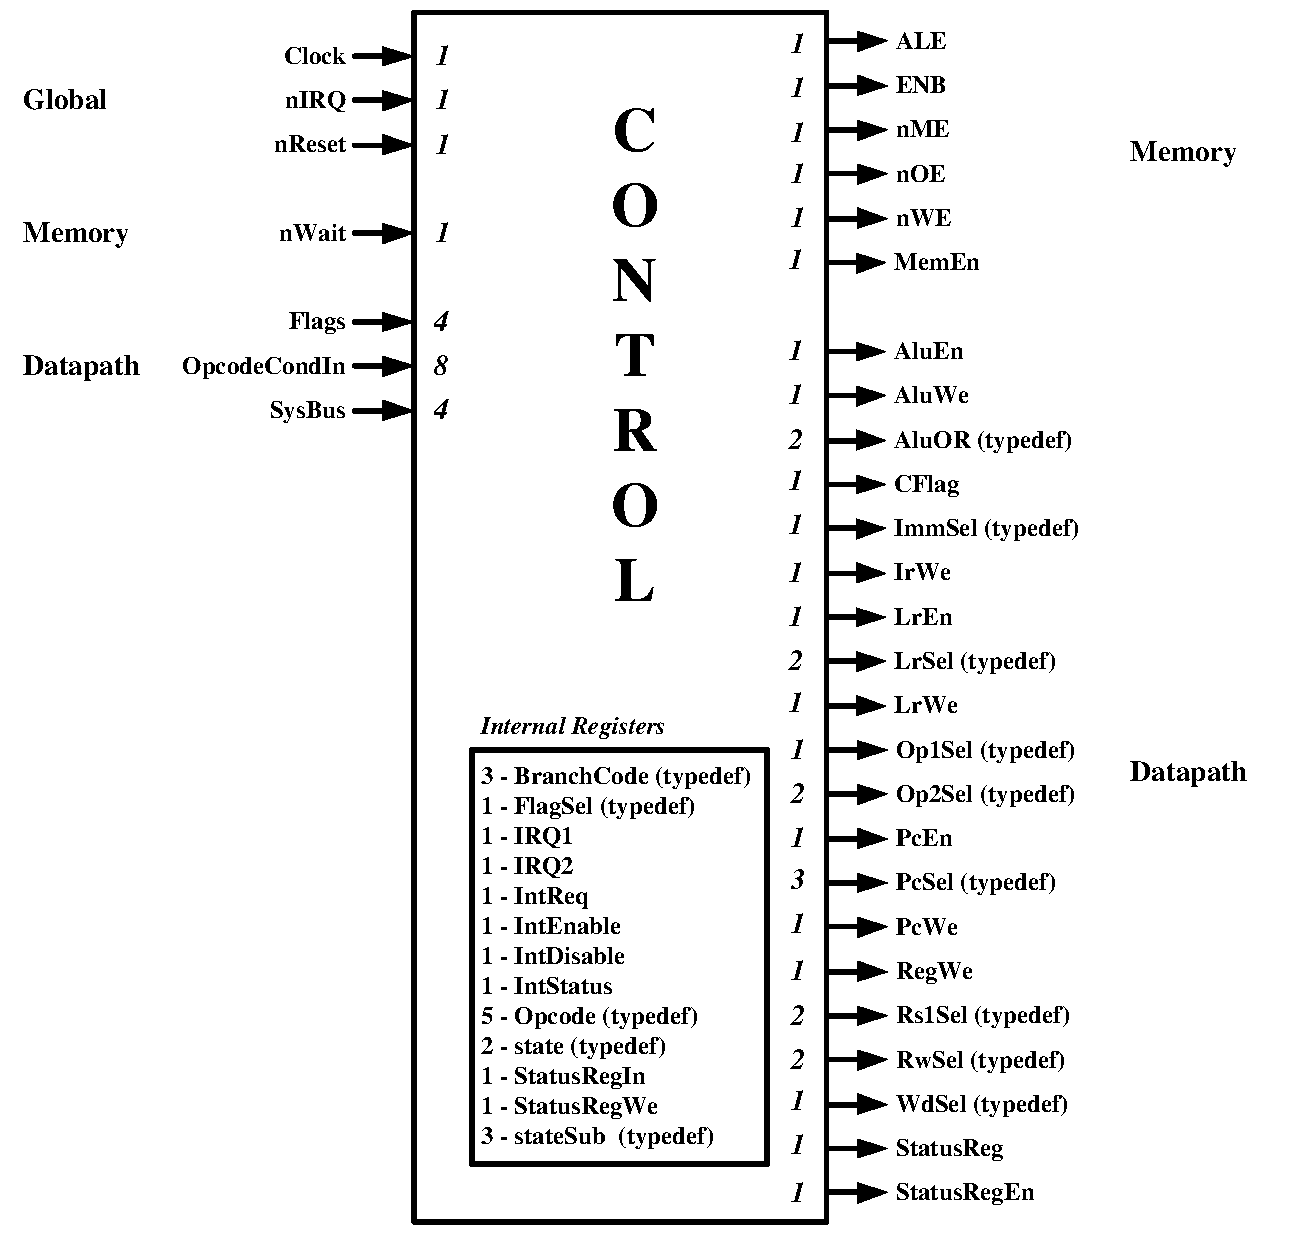
\includegraphics[width = 0.9\textwidth]{ControlPinout.pdf}
		\caption{Inputs, outputs and internal registers of the control block.}% \todo[inline]{Maybe change to IEEE symbols if we have time, AJR: we still have the eagle d-types but I think it would look a bit messy} }
   \label{fig:ControlBlock}
\end{figure}

Three main states exist to service the fetch, execute and interrupt stages.
Five sub states are used within the main states to further coordinate operation.
The ASM chart in Figure~\ref{fig:MainStateASM} describes state changes using the sub state, Opcode and interrupt request signal.   
%Linked state machines are are used to produce the 
When \textit{nReset} is asserted the machine will return to the first cycle of the fetch state.
\todo[inline]{HSL: @AJR - this has an incomplete sentence in. - now commented out.}



\begin{figure}[ht]
   \centering
    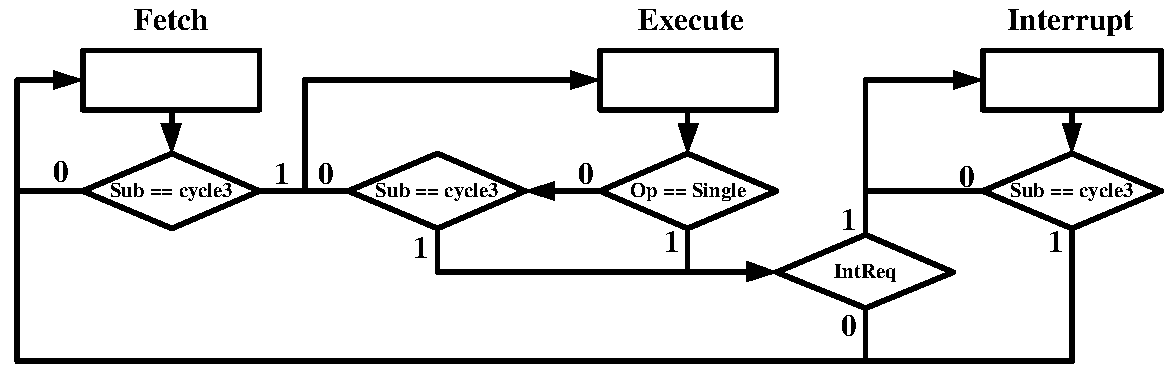
\includegraphics[width = \textwidth]{MainStateASM.pdf}
		\caption{ASM chart of controller main states.}
		\label{fig:MainStateASM}
\end{figure}








\subsection{Fetch}

Fetching an instruction from memory requires placing the program counter on the address bus then reading the instruction in to the instruction register. 
The state machine described in Figure~\ref{fig:FetchASM} asserts signals associated with memory access and delays if the slow memory access input, \textit{nWait}, is set.
When the transition from \textbf{cycle3} to \textbf{cycle0} is made the main state machine, Figure~\ref{fig:MainStateASM}, also make a transition therefore severing the link to this machine. 

\begin{figure}[ht]
   \centering
    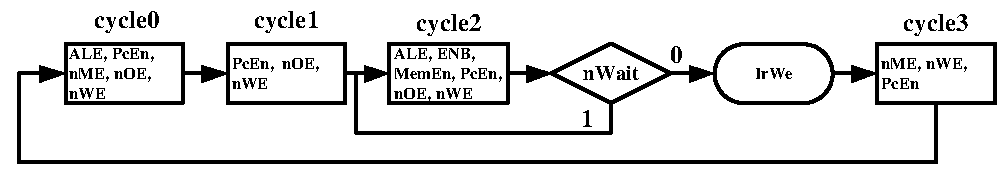
\includegraphics[width = \textwidth]{FetchASM.pdf}
		\caption{ASM chart of sub state transitions in the fetch stage.}
		\label{fig:FetchASM}
\end{figure}





\subsection{Execute}

The instruction fetched from memory is decoded in one cycle
This is a variable length stage that takes either $1$ or $4$ cycles depending on whether the instruction in the requires memory access.
After the instruction has been executed the \textit{IntReq} signal is checked to decide whether an interrupt has occurred.
\todo[inline]{HSL: @AJR - incomplete}

\begin{figure}[ht]
   \centering
    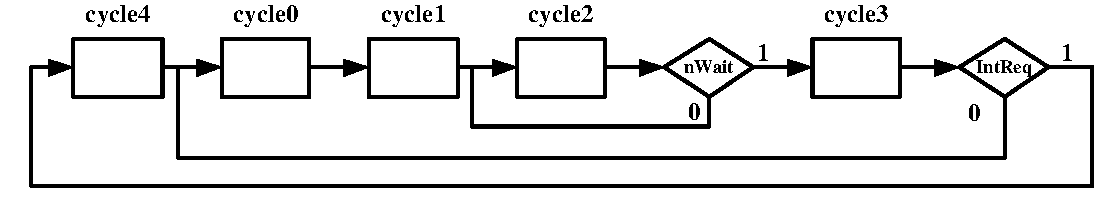
\includegraphics[width = \textwidth]{ExecuteASM.pdf}
		\caption{ASM chart of sub state transitions in the execute stage.}
		\label{fig:ExecuteASM}
\end{figure}





\subsection{Interrupt}

The circuit in Figure~\ref{fig:IntReqCircuit} is used to generate an interrupt request.
To avoid problems introduced by metastability the external \textit{nIRQ} signal is retimed using two D-types.
\textit{IntEnable} can only be set in code using the \textbf{ENAI} instruction.
\textit{IntDisable} is set when the processor is interrupted and also in code using the \textbf{DISI} instruction.
The end register contains \textit{IntStatus} which is low at reset therefore interrupts are off by default. 

\begin{figure}[ht]
   \centering
    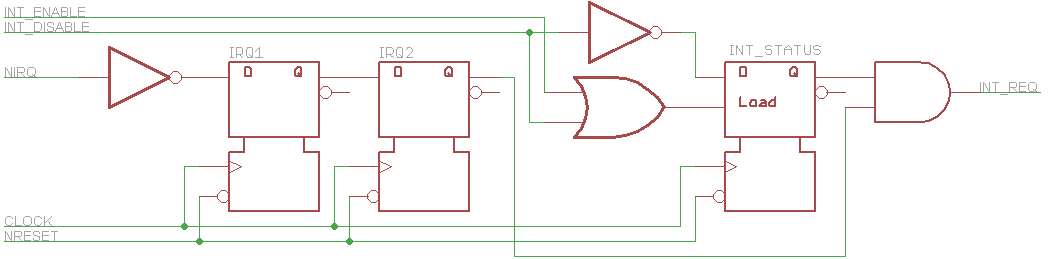
\includegraphics[width = \textwidth]{Interrupt.png}
		\caption{IntReq generation circuit.}
		\label{fig:IntReqCircuit}
\end{figure}


Entering an interrupt service routine (ISR) is completely handled in hardware. 
Interrupts are disabled and override functionality is used to decrement the stack pointer therefore allowing the program counter to be pushed to the stack.
The program counter is forced to address $0x0010$ which contains the code for ISR. 
The first operation in the ISR is \textbf{STF} which also places the flags, located in the control unit, on the stack.

The penultimate operation in the ISR should be \textbf{LDF}. This loads the flags back in to the control unit.
This is similar to a \textbf{POP} operation but writes to the control unit instead of a general purpose register. 
The final operation is a \textbf{RETI} which again is similar to a \textbf{POP}, but writes to the program counter.

A bidirectional data interface to the control unit is required to facilitate these operations. 
Figure~\ref{fig:FlagCircuit} contains the circuit used to load and store flags inside the control unit.
The $4$ bit word containing the flags is can be sourced from either the ALU or the bottom bits of SysBus. 
When storing the flags in memory the output of the status register must be placed on SysBus where the upper $12$ bits are all set to zero.

\begin{figure}[ht]
   \centering
    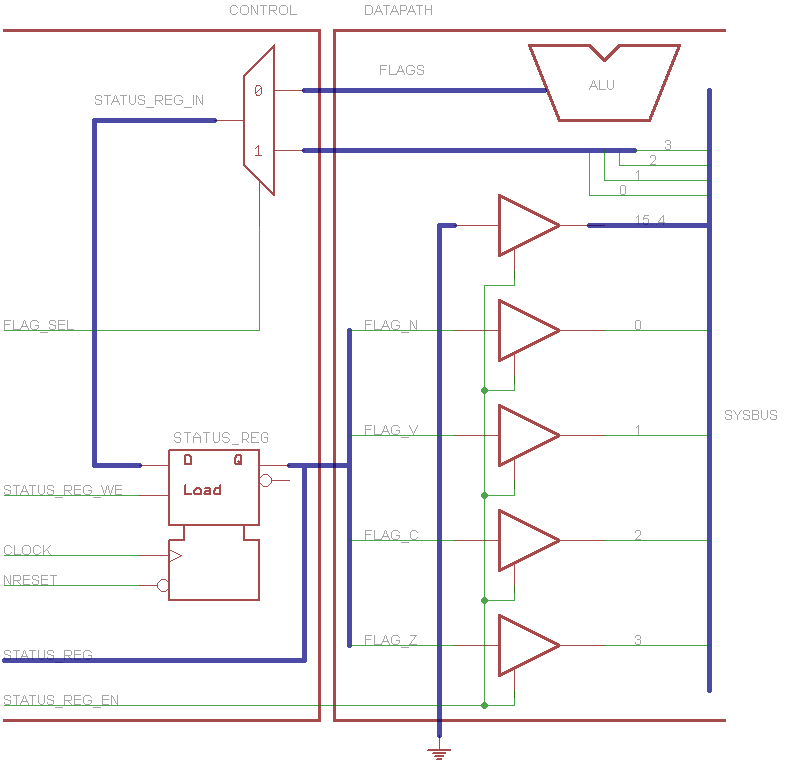
\includegraphics[width = 0.7\textwidth]{ControlIF.png}
		\caption{Control unit flag interface.}
		\label{fig:FlagCircuit}
\end{figure}





\subsection{Synthesis}

The controller was synthesised using Cadence Encounter. 
This provided a gate level netlist which was then used for place and route.
Both Magic and L-Edit place and route tools were used. 

The Magic place and route algorithm had a considerably larger routing channel than L-Edit algorithm as the cells were all placed in one long row. 
This was suboptimal as it resulted in a lot of dead space within the floorplan.

The L-Edit place and route provided far better results. 
The datapath and controller were approximately the same width. 
The I/Os were able to be positioned around the module to reduce the overall wiring needed in the full floor plan. 
Most of the datapath control signals were routed to the top of the module to reduce the wiring channel needed between the controller and datapath.
All the memory access signals were routed to the left of the controller to make easier connections to the pad ring. 
The controller was also connected to the low nibble of the input data. 
This was connected at the bottom of the controller to reduce wiring needed. 
Finally, decoder signals and flag inputs were routed to the right of the control. 


